\documentclass[]{article}
\usepackage{lmodern}
\usepackage{amssymb,amsmath}
\usepackage{ifxetex,ifluatex}
\usepackage{fixltx2e} % provides \textsubscript
\ifnum 0\ifxetex 1\fi\ifluatex 1\fi=0 % if pdftex
  \usepackage[T1]{fontenc}
  \usepackage[utf8]{inputenc}
\else % if luatex or xelatex
  \ifxetex
    \usepackage{mathspec}
  \else
    \usepackage{fontspec}
  \fi
  \defaultfontfeatures{Ligatures=TeX,Scale=MatchLowercase}
\fi
% use upquote if available, for straight quotes in verbatim environments
\IfFileExists{upquote.sty}{\usepackage{upquote}}{}
% use microtype if available
\IfFileExists{microtype.sty}{%
\usepackage{microtype}
\UseMicrotypeSet[protrusion]{basicmath} % disable protrusion for tt fonts
}{}
\usepackage[margin=1in]{geometry}
\usepackage{hyperref}
\hypersetup{unicode=true,
            pdftitle={The Migrant Crisis Effect on the EU},
            pdfauthor={Alina Kosiakova},
            pdfborder={0 0 0},
            breaklinks=true}
\urlstyle{same}  % don't use monospace font for urls
\usepackage{graphicx,grffile}
\makeatletter
\def\maxwidth{\ifdim\Gin@nat@width>\linewidth\linewidth\else\Gin@nat@width\fi}
\def\maxheight{\ifdim\Gin@nat@height>\textheight\textheight\else\Gin@nat@height\fi}
\makeatother
% Scale images if necessary, so that they will not overflow the page
% margins by default, and it is still possible to overwrite the defaults
% using explicit options in \includegraphics[width, height, ...]{}
\setkeys{Gin}{width=\maxwidth,height=\maxheight,keepaspectratio}
\IfFileExists{parskip.sty}{%
\usepackage{parskip}
}{% else
\setlength{\parindent}{0pt}
\setlength{\parskip}{6pt plus 2pt minus 1pt}
}
\setlength{\emergencystretch}{3em}  % prevent overfull lines
\providecommand{\tightlist}{%
  \setlength{\itemsep}{0pt}\setlength{\parskip}{0pt}}
\setcounter{secnumdepth}{0}
% Redefines (sub)paragraphs to behave more like sections
\ifx\paragraph\undefined\else
\let\oldparagraph\paragraph
\renewcommand{\paragraph}[1]{\oldparagraph{#1}\mbox{}}
\fi
\ifx\subparagraph\undefined\else
\let\oldsubparagraph\subparagraph
\renewcommand{\subparagraph}[1]{\oldsubparagraph{#1}\mbox{}}
\fi

%%% Use protect on footnotes to avoid problems with footnotes in titles
\let\rmarkdownfootnote\footnote%
\def\footnote{\protect\rmarkdownfootnote}

%%% Change title format to be more compact
\usepackage{titling}

% Create subtitle command for use in maketitle
\providecommand{\subtitle}[1]{
  \posttitle{
    \begin{center}\large#1\end{center}
    }
}

\setlength{\droptitle}{-2em}

  \title{The Migrant Crisis Effect on the EU}
    \pretitle{\vspace{\droptitle}\centering\huge}
  \posttitle{\par}
    \author{Alina Kosiakova}
    \preauthor{\centering\large\emph}
  \postauthor{\par}
      \predate{\centering\large\emph}
  \postdate{\par}
    \date{2019-06-17}


\begin{document}
\maketitle

INTRODUCTION

The migration crisis in the EU has led to a number of changes in the
political, economic and social environments. According to the UN,
arrivals in the year 2015 via the Mediterranean peaked at more than 1
million and polls have shown that immigrants have become voters number
one concern and in a number of countries, such as France, Germany,
Austria, Italy and Hungary, even the elections have been swayed to
popularize populist and Eurosceptic parties. There are two vastly
different opinions on the migration crisis -- some people say it is a
major threat that will destroy the EU, while others agree that it is a
necessary thing to do to helps those in need and we will benefit
massively from it in the future. In this essay, I will analyse the
available data from neutral, non-political sources and conclude how the
societies of the EU have really been affected by the migration crisis.

MAIN PART

I. What caused the migrant crisis and why did the EU become the target?

Officially we place the beginning of the migration crisis in 2015. In
reality, that year is when Europe was hit by the storm of asylum
seekers, but the trouble started brewing much earlier. The majority of
the immigrants are people from Syria, Afghanistan and Somalia. There are
multiple reasons why the immigration crisis started and why EU became
the main destination: 1) The Syrian civil war. According to the
statistics compiled by the UN, the majority of asylum seekers come from
Syria to Greece and Italy across the Mediterranean Sea. The people are
afraid of war and run to protect themselves and their families from
death -- a very understandable fear and need. The reason why Europe is
so attractive to them is because of legalities. The Syrian refugees who
have immigrated to other Arab countries do not have the right to work,
are not recognised as refugees and many of their children do not have
access to basic education. Data provided by the UN shows that around
400000 Syrian children that are currently living in Turkey were rejected
from the education system. Also, there has been a cut in UN funding
which led to decreased financial help to Syrian families which makes the
Middle East a highly unattractive place for people to stay. 2)
Encouragement from German Chancellor Angela Merkel. The EU laws say that
the country to which an asylum seeker arrives first is the one held
responsible for their application and resettling them, that is why
countries such as Italy, Greece and Malta were heavily burdened by
helping the refugees. A new wave of asylum seekers hit Europe when it
was declared that if they manage to reach Germany, they could
effectively apply for asylum there. 3) Self-perpetuating element. The
refugees that are lucky enough to reach Europe consequentially encourage
their friends and families to try and immigrate to the EU as well. Also,
the media's intensive coverage on brief gaps in border control or
impending caps on refugee numbers increase the number of people willing
to try their luck as asylum seekers. 4) Poverty and turmoil in
sub-Saharan Africa. Many countries in that area of the continent are
underdeveloped and poor. Before the instability in Libya, people would
move there to find jobs and help their families, but now more people try
to cross the Mediterranean.

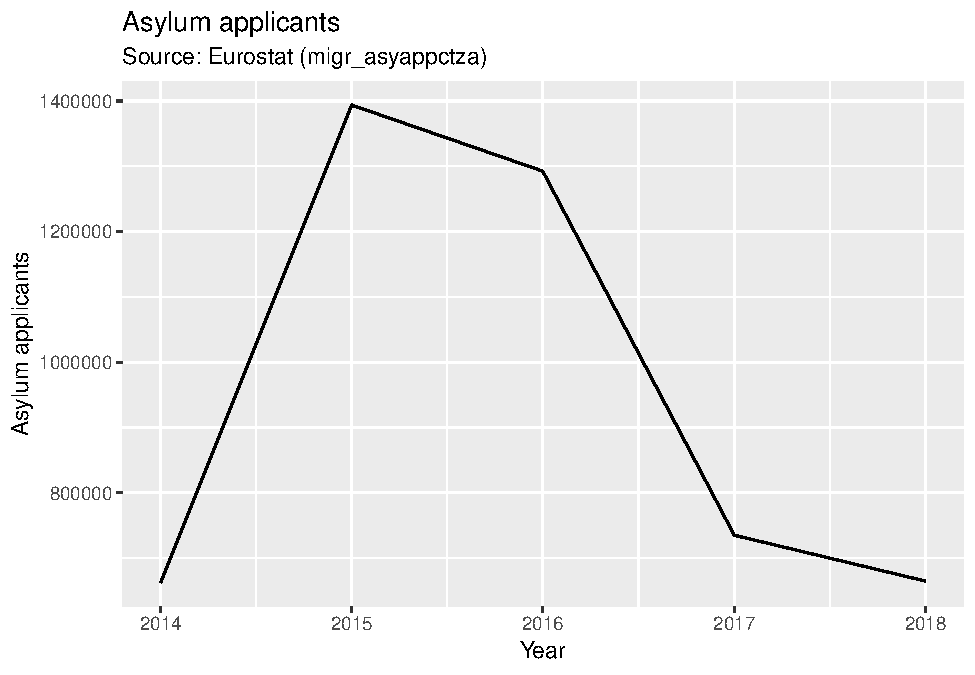
\includegraphics{Alina_files/figure-latex/unnamed-chunk-4-1.pdf} II.
What kind of effect did the migrant crisis have on the economy of the
EU?

The potential effect of the migration crisis on the economy is still
very much up in the air. Many people are concerned that it might in fact
weaken the economy by increasing unemployment, overloading the public
budgets and straining the infrastructural capacity. Also, there is a
fear that the refugee crisis will worsen the debt crisis. But is that
really the case? We can divide the effects to short-term and long-term.
1) Short-term. According to economist O. Reynolds, the short-term
effects will be positive, but only slightly. When a refugee arrives to
the host country, their health problems should be checked, children and
adults must be educated to integrate them into the work labour markets,
and also, financial support is required to help them before the adults
are fully prepared to support their families. The cost to integrate a
refugee into society varies from 8000 euros to 12000 euros per
application (Kern, 2015). It means that the fiscal costs will come
before the fiscal benefits for the host countries, but that will give an
immediate positive boost to domestic demand. As stated in IMF, by the
end of 2017 the GDP in Austria, Germany and Sweden -- these countries
have accommodated the most of refugees -- had grown by 0.5\%, 0.3\% and
0.4\%, respectively. According to The Economist, economic analysis
demonstrates that the migrant increase will not increase the
unemployment or decrease the wages of the already working native
population.

\begin{enumerate}
\def\labelenumi{\arabic{enumi})}
\setcounter{enumi}{1}
\tightlist
\item
  Long-term. The results of the migration crisis are hard to predict.
  Not only because nothing major as this has not happened since World
  War II, but also because little is known about the education level and
  capabilities of the ones who have already immigrated to Europe. The
  process also heavily depends on how countries will be able to present
  the refugees to the work force and help them throughout the process of
  integration. In fact, the government only starts to receive fiscal
  benefits when the refugees enter the labour market. Also, the refugee
  crisis might be the solution to help an aging Europe with their
  declining birth-rate as the migrants will become net payers and
  contribute towards the increasing welfare expenditure on the
  pensioners. As of now, the current tendencies of gaining demographics
  will slow down the economic growth of Central Europe and Baltic
  nations. By welcoming the refugees, many of whom are young and
  skilled, may prove to be a lifeline for these economies because it
  would increase the number of people employed and contributing to the
  welfare system. Moreover, local businesses have reported that they
  received an increase in turnover and profits attributed to purchases
  made by the support staff, refugee customers and those engaged in
  public works. Refugees also tend to open their own small businesses
  according to information from Austria, Bulgaria and Sweden. The only
  problem remains -- it is hard for businesses to employ asylum seekers
  and refugees due to their unclear residence status, language skills,
  level of qualifications, professional training and support needs, the
  recognition of diplomas, the lack of affordable housing and transport,
  xenophobia and bureaucratic hurdles for employers.
\end{enumerate}

\begin{enumerate}
\def\labelenumi{\Roman{enumi}.}
\setcounter{enumi}{2}
\tightlist
\item
  How did the migrant crisis change the political stances and the
  societies of the EU?
\end{enumerate}

The biggest challenge in fact is the political climate of Europe. The
migrant crisis consequentially led to the split between the older EU
members such a Germany and the newer Central and Eastern European
members. For example, they are divided on the quota system for refugee
allocation to different EU counties. The debate among Member States had
clearly demonstrated our differences not only in terms of fulfilling the
EU obligations but also in the understanding of the value of human
rights protection. Based on the scenarios that the European Commission
has created (2017), it seems almost certain that their adoption will
soon lead to the establishment of two different sides of the European
Union. One of them will be the core, including Germany and hopefully
France as leaders, and they would work to deepen their integration.
Consequently, the so called ``core'' would diminish the role of
countries which do not follow European obligations and fundamental
rules. This poses a great threat to those countries, as this group
includes the new Member States that benefit directly from the European
integration process in the area of the Cohesion Policy, free movement of
goods, services or capital. In the coming years they may become just a
gateway to the European Union. Should that occur, the disintegration
process will start, as for a Member State to become simply an entryway
to the common market would be tantamount to EU's disintegration. The
people have drastically different views on the migration crisis.
According to Barysch, 2016, in a poll conducted in 2015, 60-80\% of
people in France, Italy, Spain and the UK claim they are displeased with
their government's immigration policies. Another poll in 2016 showed
that 61\% in France, 71\% in Greece and 48\% in the UK have feelings
that their country's membership in the EU is unfavourable in the current
situation (Arnett 2016). These increasingly high numbers clearly
indicate that the European citizens support the rise of right-wing,
anti-EU and xenophobic political parties in many EU countries. For
example, the far-right Conservative People's Party of Estonia has almost
18\% of votes in 2018, making in the third-largest part and Germany's
far-right party Alternative for Germany (AfG) entered the federal
parliament for the first time with 12,6\% of the votes and they became
the biggest opposition party in the country. That explains the reasons
why the wave of xenophobia has covered Europe. Never before have the
European citizens been so sceptical about the European Union and its
leaders. Hostility and mistrust have increased even in the most tolerant
communities. Reception centres have met resistance in Denmark, Slovakia
and Sweden and xenophobia and racism have become increasingly socially
acceptable over social media.

CONCLUSION The migrant crisis has become and will be one of the main
problems of the European Union for quite some time. The findings of
economist and finance analysts have shown that the refugee crisis might
actually benefit Europe as a whole, not only increasing our turnover,
but also helping an aging Europe. There will be challenges to integrate
those people into society and help them find their way in the labour
market, but the long-term benefits clearly outweigh the drawbacks. When
it comes to the political consequences, it is clear that the EU is far
from being integrated and the different Member States have drastically
opposite opinions on the matter which rises from the general
unsatisfaction of the general public who have started to support
right-wing and sometimes even racist political parties, creating a more
dangerous place for asylum seekers in Europe. It is clear that the EU
will keep supporting the migrant crisis if the leaders of the union
(Germany and France) have pro-migrant leaders. And only time will tell
what happens next.

Poddar (2016) Fundamental Rights (2018) ({\textbf{???}}) Borowicz (2017)
({\textbf{???}}) Herm and Poulain (2018) Oliver Reynolds (2017)
Elizabeth Collett (n.d.)

\hypertarget{references}{%
\subsection*{References}\label{references}}
\addcontentsline{toc}{subsection}{References}

\hypertarget{refs}{}
\leavevmode\hypertarget{ref-aleksandraborowicz2017}{}%
Borowicz, Aleksandra. 2017. ``The European Migration Crisis -- Economic
and Political Factors and Challenges for the Future.'' \emph{University
of Gdańsk}.

\leavevmode\hypertarget{ref-elizabethcollettcamillelecoz}{}%
Elizabeth Collett, Camille Le Coz. n.d. ``After the Storm.''
\emph{Migration Policy Institute Europe}.

\leavevmode\hypertarget{ref-europeanunionagencyforfundamentalrights2018}{}%
Fundamental Rights, European Union Agency for. 2018. ``Current Migration
Situation in the Eu: Impact on Local Communities (Update).'' \emph{FRA
-- EUROPEAN UNION AGENCY FOR FUNDAMENTAL RIGHTS}.

\leavevmode\hypertarget{ref-annehermmichelpoulain2018}{}%
Herm, Anne, and Michel Poulain. 2018. ``Economic Crisis and
International Migration. What the Eu Data Reveal?'' \emph{Migration et
Confection}, p. 145--69.

\leavevmode\hypertarget{ref-oliverreynolds2017}{}%
Oliver Reynolds. 2017. ``Bounty or Burden? The Impact of Refugees on
European Economies Is Far from Clear.'' \emph{FocusEconomics}.

\leavevmode\hypertarget{ref-shubhampoddar2016}{}%
Poddar, Shubham. 2016. ``European Migrant Crisis: Financial Burden or
Economic Opportunity?'' \emph{Social Impact Research Experience (SIRE)}.


\end{document}
